% Provenance (never printed): see sources/outline_sources.md (Year 1:
% the Solar System, planetology). Kepler's laws, the moment of inertia and
% the Stefan--Boltzmann law are owned by the physics series and recalled
% here; the equilibrium temperature and the Bond albedo are re-founded from
% Book 2 grade 10. Curves computed in figdata/bachelor-1/planet_table.py;
% numbers of the exercises and problem in the Book 3 scratch calculator
% ch03.py.
\chapter{Planetologi komparatif}\label{ch:b1:comparative-planetology}

Venus dan Bumi hampir kembar: Venus memiliki \qty{95}{\percent} jari-jari Bumi dan \qty{81}{\percent} massanya. Namun Bumi memiliki samudra, atmosfer nitrogen--oksigen, dan lempeng-lempeng yang bergerak, sedangkan Venus bersembunyi di balik awan dengan permukaan bersuhu \qty{737}{K}, lebih panas daripada oven dapur mana pun, tertekan oleh atmosfer karbon dioksida pada \qty{92}{bar}. Mars, yang setengah ukuran Bumi, memiliki atmosfer tipis yang dingin, gunung api raksasa dan ngarai, tetapi tidak ada lempeng yang bergerak. Lebih jauh, Jupiter dan Saturnus sebagian besar terdiri atas hidrogen dan helium; Uranus dan Neptunus sebagian besar terdiri atas es air, metana, dan amonia. Membandingkan planet adalah satu-satunya cara untuk menguji apa yang kita kira kita ketahui tentang Bumi: mengapa bagian dalamnya berlapis, mengapa iklimnya sedang, mengapa hanya Bumi yang memiliki tektonik lempeng. Bab ini menimbang dan mengukur planet-planet, membaca bagian dalamnya dari massa jenis dan cara massanya terdistribusi, membandingkan suhu dan atmosfernya, dan berakhir dengan bulan-bulan serta benda-benda kecil yang menyimpan catatan masa muda Tata Surya.
% ledger: nasa:venus, earth:Rmean, earth:mass, nasa:uranus-structure

\begin{recall}
Planet-planet mengelilingi Matahari pada elips, dan kuadrat periode satelit sebanding dengan pangkat tiga sumbu semi-major-nya (hukum ketiga Kepler, dalam volume Sarjana Tahun ke-1 buku fisika, tempat momen inersia benda padat juga didefinisikan; sebuah bola seragam memiliki $I = \tfrac25MR^2$). Benda hitam memancarkan $\sigma T^4$ per satuan luas (Sarjana Tahun ke-2). Tata Surya serta planet-planet batuan dan raksasa diuraikan dalam Buku 1 (kelas 6); albedo dan \omterm{def:b1:comparative-planetology:equilibrium-temperature}{suhu kesetimbangan} suatu planet telah dijumpai di Buku 2 (kelas 10), dan efek rumah kaca di Buku 1 (kelas 9).
\end{recall}

\begin{omfigure}
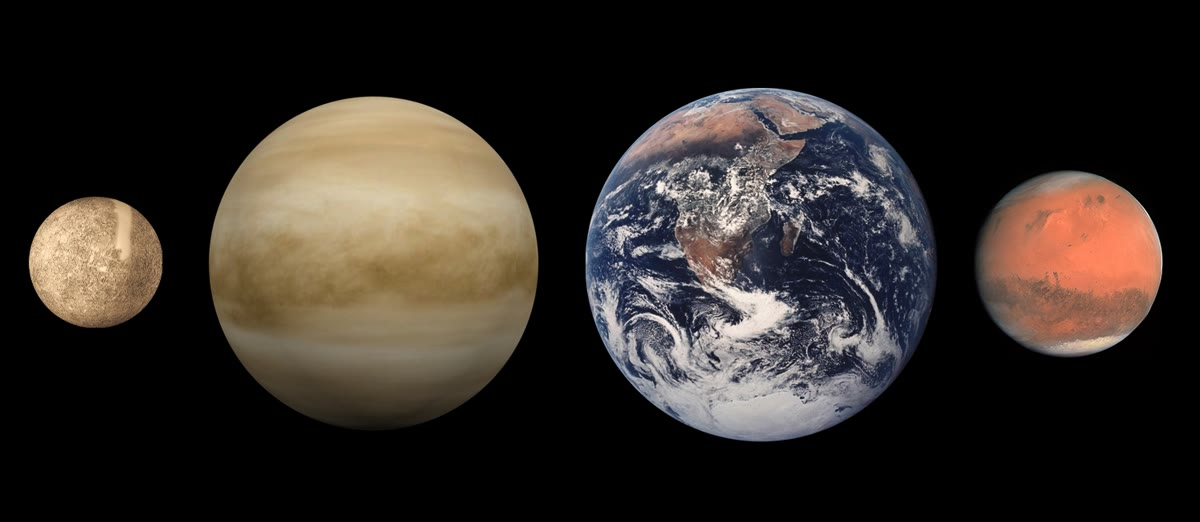
\includegraphics[width=0.85\linewidth]{images/book3/b1-terrestrial-planet-sizes.jpg}

{\small Empat \omterm{def:b1:comparative-planetology:planet-types}{planet terestrial} dalam skala, dari kiri ke kanan Merkurius, Venus, Bumi dan Mars (jarak tidak sesuai skala; Venus tampak dalam cahaya tampak, permukaannya tersembunyi di balik awan). NASA, domain publik.}
% ledger: commons:terrestrial-sizes
\end{omfigure}

\section{Menimbang dan mengukur planet}

Jari-jari planet diukur dari diameter sudut dan jaraknya, atau, untuk planet yang dikunjungi wahana antariksa, dari altimetri radar dan laser. Massanya lebih sulit: ia hanya dirasakan melalui gaya gravitasi yang dikerjakan planet itu pada sesuatu yang lain.

\begin{method}[Massa planet dari orbit satelit]\label{met:b1:comparative-planetology:mass}
Untuk satelit bermassa yang dapat diabaikan pada orbit hampir lingkaran dengan jari-jari (sumbu semi-major) $a$ dan periode sideris $T$ mengelilingi planet bermassa $M$:
\begin{enumerate}
  \item ubahlah $a$ ke meter dan $T$ ke detik;
  \item hukum ketiga Kepler memberikan $GM = 4\pi^2a^3/T^2$: hasil kali ini adalah yang diukur oleh orbit, dengan ketelitian jauh lebih baik daripada $G$ itu sendiri;
  \item bagilah dengan $G = \qty{6.6743e-11}{m^3.kg^{-1}.s^{-2}}$ untuk memperoleh $M$.
\end{enumerate}
Planet tanpa bulan (Merkurius, Venus) ditimbang dengan cara yang sama dari orbit, atau dari pembelokan sebuah wahana antariksa yang melintas di dekatnya.
\end{method}

\begin{example}
Io, bulan besar terdalam Jupiter, mengorbit pada $a = \qty{421.8e3}{km}$ dalam \num{1.769138} hari, yaitu $T = \qty{152854}{s}$. Maka
\[
  GM = \frac{4\pi^2\times(\qty{4.218e8}{m})^3}{(\qty{152854}{s})^2}
  = \qty{1.268e17}{m^3.s^{-2}}, \qquad
  M = \frac{\num{1.268e17}}{\num{6.6743e-11}} = \qty{1.900e27}{kg},
\]
yang sesuai dengan massa Jupiter dalam tabel, \qty{1.898e27}{kg}, hingga \qty{0.1}{\percent}. Massa Io sendiri, \num{4.7e-5} massa Jupiter, dapat diabaikan; kelebihan kecil itu berasal dari penggembungan khatulistiwa Jupiter, yang menarik bulan dekat sedikit lebih kuat daripada bola bermassa sama.
% ledger: nasa:io, nasa:jupiter, const:G
\end{example}

Dari massa dan jari-jari diperoleh massa jenis rata-rata $\bar\rho =
3M/(4\pi R^3)$, petunjuk pertama tentang bahan pembentuk planet. Massa jenis planet-planet terbagi dalam dua kelompok (lihat gambar di bawah): Merkurius, Venus, Bumi dan Mars berada antara sekitar \num{3900} dan \qty{5500}{kg.m^{-3}}, lebih padat daripada batuan umum mana pun; keempat planet luar berada antara \num{690} dan \qty{1640}{kg.m^{-3}}, mendekati massa jenis air, dan Saturnus bahkan di bawahnya.
% ledger: planet:Mercury.density, planet:Mars.density, planet:Earth.density, planet:Saturn.density, planet:Neptune.density

\begin{omfigure}
\begin{tikzpicture}
\begin{axis}[omrecord, width=0.86\linewidth, height=6.2cm, xmode=log,
  xmin=800, xmax=150000, ymin=0, ymax=6300, xlabel={jari-jari khatulistiwa (km)},
  ylabel={massa jenis rata-rata (\unit{kg.m^{-3}})}, tick label style={font=\scriptsize},
  label style={font=\small}]
\addplot[only marks, mark=*, mark size=2.4pt, brown!70!black] table[x=R_km, y=density,
  restrict expr to domain={\thisrow{idx}}{0:2}] {figdata/out/bachelor-1-planet_table-bodies.dat};
\addplot[only marks, mark=*, mark size=2.4pt, brown!70!black] table[x=R_km, y=density,
  restrict expr to domain={\thisrow{idx}}{4:4}] {figdata/out/bachelor-1-planet_table-bodies.dat};
\addplot[only marks, mark=*, mark size=2.4pt, orange!85!black] table[x=R_km, y=density,
  restrict expr to domain={\thisrow{idx}}{5:6}] {figdata/out/bachelor-1-planet_table-bodies.dat};
\addplot[only marks, mark=*, mark size=2.4pt, omDef] table[x=R_km, y=density,
  restrict expr to domain={\thisrow{idx}}{7:8}] {figdata/out/bachelor-1-planet_table-bodies.dat};
\addplot[only marks, mark=o, mark size=2.4pt, black!60] table[x=R_km, y=density,
  restrict expr to domain={\thisrow{idx}}{3:3}] {figdata/out/bachelor-1-planet_table-bodies.dat};
\addplot[only marks, mark=o, mark size=2.4pt, black!60] table[x=R_km, y=density,
  restrict expr to domain={\thisrow{idx}}{9:9}] {figdata/out/bachelor-1-planet_table-bodies.dat};
\addplot[black!40, densely dashed] coordinates {(800,1000) (150000,1000)};
\begin{scope}[font=\scriptsize]
\node[left] at (axis cs:2439.5,5429) {Merkurius};
\node[below left] at (axis cs:6052,5243) {Venus};
\node[above] at (axis cs:6378,5514) {Bumi};
\node[left] at (axis cs:3396,3934) {Mars};
\node[left] at (axis cs:1737.5,3340) {Bulan};
\node[right] at (axis cs:1188,1850) {Pluto};
\node[above] at (axis cs:71492,1326) {Jupiter};
\node[left] at (axis cs:60268,687) {Saturnus};
\node[right] at (axis cs:25559,1270) {Uranus};
\node[above] at (axis cs:24764,1638) {Neptunus};
\node[above left, black!60] at (axis cs:150000,1000) {air};
\end{scope}
\end{axis}
\end{tikzpicture}

{\small Massa jenis rata-rata terhadap jari-jari (logaritmik) untuk kedelapan planet (terisi: \omterm{def:b1:comparative-planetology:planet-types}{planet terestrial}, \omterm{def:b1:comparative-planetology:planet-types}{raksasa gas}, \omterm{def:b1:comparative-planetology:planet-types}{raksasa es}), Bulan dan Pluto (lingkaran terbuka). Data dari lembar fakta planet NASA.}
% ledger: planet:Mercury.diameter, planet:Venus.diameter, planet:Earth.diameter, planet:Moon.diameter, planet:Mars.diameter, planet:Jupiter.diameter, planet:Saturn.diameter, planet:Uranus.diameter, planet:Neptune.diameter, planet:Pluto.diameter, planet:Mercury.density, planet:Venus.density, planet:Earth.density, planet:Moon.density, planet:Mars.density, planet:Jupiter.density, planet:Saturn.density, planet:Uranus.density, planet:Neptune.density, planet:Pluto.density
\end{omfigure}

Massa jenis rata-rata saja tidak dapat memberi tahu apakah sebuah planet terbuat dari satu bahan yang padat, atau dari planet dengan pusat yang sangat padat dan selubung yang lebih ringan. Sebuah bilangan kedua memberi tahu: bagaimana massanya terdistribusi antara pusat dan permukaan.

\begin{definition}[Faktor momen inersia]\label{def:b1:comparative-planetology:moi}
Yang disebut \emph{faktor momen inersia}\index{faktor momen inersia} suatu planet adalah bilangan
\[
  C = \frac{I}{MR^2} ,
\]
dengan $I$ momen inersianya terhadap sumbu rotasi, $M$ massanya, dan $R$ jari-jari rata-ratanya. Bola seragam memiliki $C = \tfrac25 = 0.4$; planet yang massa jenisnya bertambah ke arah pusat memiliki $C < 0.4$, makin kecil nilainya makin terkonsentrasi massanya.
\end{definition}

Momen inersia diukur dari presesi lambat sumbu rotasi di bawah tarikan Matahari, bersama dengan pemipihan medan gravitasi planet. Nilainya mengungkapkan: Bulan, $C = 0.394$, hampir seragam; Mars, $0.366$, dan Bumi, $0.3308$, jelas berlapis; Jupiter, $0.254$, dan Saturnus, $0.210$, memiliki sebagian besar massanya terkemas ke arah pusatnya.
% ledger: nasa:moon, nasa:mars, earth:MoI, nasa:jupiter, nasa:saturn

\section{Bahan pembentuk planet}

\begin{definition}[Planet terestrial dan raksasa]\label{def:b1:comparative-planetology:planet-types}
Yang disebut \emph{planet terestrial}\index{planet terestrial} adalah planet yang sebagian besar tersusun dari batuan silikat dan besi, dengan permukaan padat: Merkurius, Venus, Bumi dan Mars. \emph{Planet raksasa}\index{planet raksasa} adalah planet yang banyak kali lebih massif daripada Bumi, sebagian besar tersusun dari unsur ringan dan senyawanya, dan tanpa permukaan padat. \emph{Raksasa gas}\index{raksasa gas} adalah planet raksasa yang sebagian besar tersusun dari hidrogen dan helium: Jupiter dan Saturnus. \emph{Raksasa es}\index{raksasa es} adalah planet raksasa yang sebagian besar tersusun dari senyawa yang oleh para astronom disebut es --- air, metana, dan amonia --- di bawah selubung hidrogen dan helium: Uranus dan Neptunus.
\end{definition}

Atmosfer yang diukur oleh wahana dan teleskop menegaskan pembagian itu. Atmosfer Jupiter \qty{89.8}{\percent} hidrogen dan \qty{10.2}{\percent} helium menurut volume, Saturnus \qty{96.3}{\percent} dan \qty{3.25}{\percent}; untuk Uranus, sekurang-kurangnya \qty{80}{\percent} massanya adalah cairan padat panas berupa air, metana, dan amonia di atas inti batuan kecil. Massa jenis rata-rata \omterm{def:b1:comparative-planetology:planet-types}{raksasa gas} tetap rendah meskipun pusatnya sangat terkompresi, karena hidrogen adalah unsur paling ringan; \omterm{def:b1:comparative-planetology:planet-types}{raksasa es} lebih padat daripada Saturnus karena es-nya lebih berat daripada hidrogen.
% ledger: nasa:jupiter, nasa:saturn, nasa:uranus-structure

Planet-planet terestrial berlapis seperti Bumi: inti kaya besi di bawah mantel silikat dan kerak tipis. Model paling sederhana yang memakai kedua bilangan terukur, massa jenis rata-rata dan \omterm{def:b1:comparative-planetology:moi}{faktor momen inersia}, memiliki dua lapisan.

\begin{proposition}[Planet dua lapis]\label{prop:b1:comparative-planetology:two-layer}
Modelkan planet berjari-jari $R$ sebagai inti berjari-jari $xR$ dan massa jenis seragam $\rho_c$ di dalam mantel bermassa jenis seragam $\rho_m$. Massa jenis rata-ratanya dan \omterm{def:b1:comparative-planetology:moi}{faktor momen inersianya} adalah
\[
  \bar\rho = \rho_m + (\rho_c - \rho_m)\,x^3 , \qquad
  C = \frac25\,\frac{\rho_m + (\rho_c - \rho_m)\,x^5}{\bar\rho} .
\]
Diberikan $\bar\rho$, $C$, dan massa jenis mantel yang diasumsikan $\rho_m$, jari-jari inti relatif mengikuti:
\[
  x^2 = \frac{\tfrac52C\bar\rho - \rho_m}{\bar\rho - \rho_m} ,
  \qquad \rho_c = \rho_m + \frac{\bar\rho - \rho_m}{x^3} .
\]
\end{proposition}

\begin{proof}
Planet adalah bola seragam bermassa jenis $\rho_m$ dan jari-jari $R$ ditambah sebuah bola berjari-jari $xR$ dengan kelebihan massa jenis $\rho_c - \rho_m$. Massa-massa dijumlahkan: $M = \tfrac43\pi R^3[\rho_m + (\rho_c - \rho_m)x^3]$, dan membaginya dengan volume memberikan $\bar\rho$. Momen inersia terhadap sumbu yang sama juga dijumlahkan; sebuah bola seragam bermassa jenis $\rho$ dan jari-jari $r$ memiliki
$I = \tfrac25\cdot\tfrac43\pi\rho r^3\cdot r^2 = \tfrac{8\pi}{15}\rho r^5$,
sehingga $I = \tfrac{8\pi}{15}R^5[\rho_m + (\rho_c - \rho_m)x^5]$. Membagi dengan
$MR^2 = \tfrac43\pi\bar\rho R^5$ menghasilkan $C$. Akhirnya kedua persamaan berbunyi
$(\rho_c - \rho_m)x^3 = \bar\rho - \rho_m$ dan $(\rho_c - \rho_m)x^5 =
\tfrac52C\bar\rho - \rho_m$; membagi persamaan kedua dengan yang pertama menghasilkan $x^2$,
dan yang pertama menghasilkan $\rho_c$.
\end{proof}

Model ini memiliki tiga besaran tak diketahui dan dua data, sehingga salah satunya, massa jenis mantel, harus diasumsikan dari apa yang ditimbang oleh batuan berkomposisi yang tepat di bawah tekanan. Jawabannya peka terhadap pilihan itu bila $C$ mendekati $0.4$, karena $\tfrac52C\bar\rho - \rho_m$ ketika itu merupakan selisih kecil dari bilangan-bilangan besar (\cref{exo:b1:comparative-planetology:10} dan soal). Model juga mengabaikan pemampatan mantel oleh beratnya sendiri, yang pada planet sebesar Bumi menaikkan massa jenis mantel dalam jauh di atas massa jenis batuan permukaan; untuk Bumi, seismologi jauh lebih baik (\cref{ch:b1:layered-earth}). Seismometer yang ditempatkan di Mars kini telah melakukan hal yang sama untuk planet itu: jika tabel planet memberikan jari-jari inti \qty{1830}{km}, hasil terbaru menunjukkan hanya \qty{1650}{km} sampai \qty{1675}{km}.
% ledger: nasa:mars-core

\begin{omfigure}
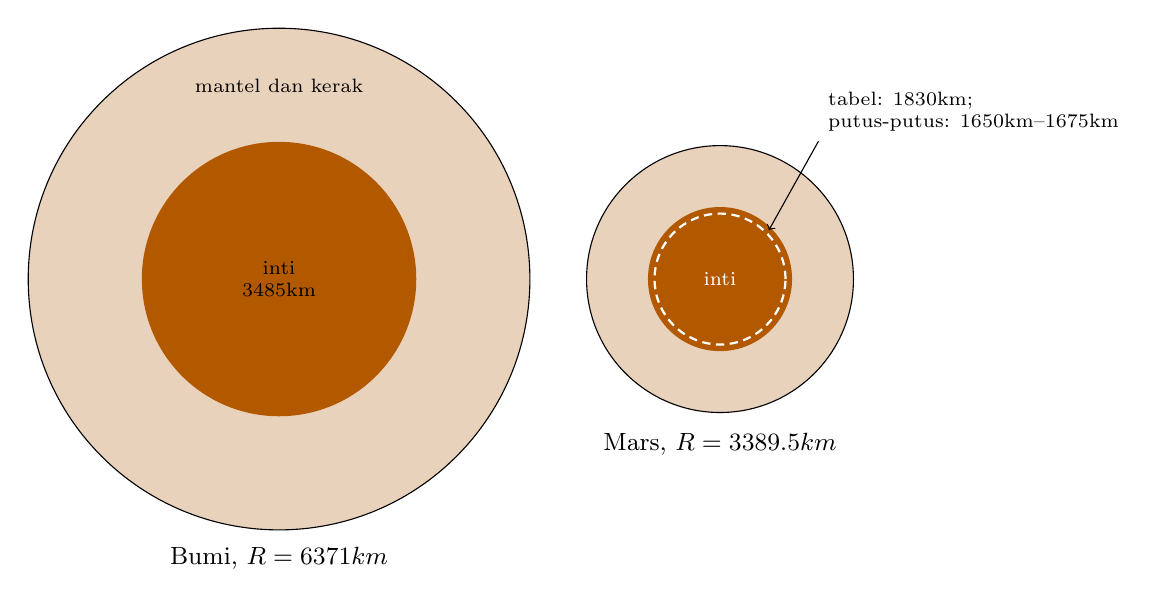
\begin{tikzpicture}[font=\scriptsize]
% scale: 0.5 cm per 1000 km
\fill[brown!35] (0,0) circle (3.1855cm);
\fill[orange!70!black] (0,0) circle (1.7425cm);
\draw (0,0) circle (3.1855cm);
\node[align=center] at (0,0) {inti\\ \qty{3485}{km}};
\node[align=center] at (0,2.45) {mantel dan kerak};
\node at (0,-3.55) {\small Bumi, $R = \qty{6371}{km}$};
\begin{scope}[xshift=5.6cm]
\fill[brown!35] (0,0) circle (1.6948cm);
\fill[orange!70!black] (0,0) circle (0.915cm);
\draw[white, densely dashed, thick] (0,0) circle (0.8313cm);
\draw (0,0) circle (1.6948cm);
\node[align=center, white] at (0,0) {inti};
\node at (0,-2.1) {\small Mars, $R = \qty{3389.5}{km}$};
\draw[->] (1.25,1.75) node[above right, align=left] {tabel: \qty{1830}{km};\\ putus-putus: \qty{1650}{km}--\qty{1675}{km}} -- (0.62,0.62);
\end{scope}
\end{tikzpicture}

{\small Bumi dan Mars dalam skala, dengan intinya. Untuk Mars, tepi padat adalah jari-jari inti dari tabel planet dan lingkaran putus-putus adalah jari-jari yang lebih kecil yang diindikasikan oleh hasil seismik terbaru. Kedua inti kaya besi; inti Bumi memiliki bagian dalam yang padat, yang tidak digambar.}
% ledger: earth:Rmean, earth:Rcore, nasa:mars, nasa:mars-core
\end{omfigure}

\section{Atmosfer dan permukaan}

Suhu planet pertama-tama ditentukan oleh cahaya Matahari yang diserapnya. Iradiansi $S$ pada jarak $d$ dari Matahari berkurang sebagai $1/d^2$ (\cref{prop:b1:observing-the-sky:inverse-square}): \qty{1361}{W.m^{-2}} di Bumi, \qty{2601}{W.m^{-2}} di Venus, \qty{586}{W.m^{-2}} di Mars, \qty{50}{W.m^{-2}} di Jupiter. Sebagian darinya dipantulkan lurus kembali.
% ledger: earth:TSI, nasa:venus, nasa:mars, nasa:jupiter

\begin{definition}[Albedo Bond]\label{def:b1:comparative-planetology:albedo}
Yang disebut \emph{albedo Bond}\index{albedo Bond} $A$ suatu planet adalah pecahan dari daya total cahaya Matahari yang jatuh padanya yang dipantulkan dan dihamburkan kembali ke angkasa, pada semua panjang gelombang dan semua arah.
\end{definition}

Salju segar dan awan terang memantulkan banyak, batuan gelap dan laut terbuka sedikit. Venus, yang terbungkus awan terang, memiliki $A = 0.77$; Bumi $0.294$; Mars $0.250$; Bulan, batuan abu-abu gelap, $0.11$.
% ledger: nasa:venus, earth:albedo, nasa:mars, nasa:moon

\begin{definition}[Suhu kesetimbangan]\label{def:b1:comparative-planetology:equilibrium-temperature}
Yang disebut \emph{suhu kesetimbangan}\index{suhu kesetimbangan} $T_\mathrm{eq}$ suatu planet adalah suhu seragam tempat sebuah benda hitam seukuran planet itu memancarkan ke angkasa tepat daya yang diserap planet dari Matahari.
\end{definition}

\begin{proposition}[Rumus suhu kesetimbangan]\label{prop:b1:comparative-planetology:teq}
Planet dengan \omterm{def:b1:comparative-planetology:albedo}{albedo Bond} $A$ yang menerima iradiansi $S$ memiliki
\[
  T_\mathrm{eq} = \left(\frac{S(1 - A)}{4\sigma}\right)^{1/4},
  \qquad \sigma = \qty{5.6704e-8}{W.m^{-2}.K^{-4}} .
\]
\end{proposition}

\begin{proof}
Planet mencegat cahaya Matahari yang jatuh pada penampangnya, sebuah cakram berluas $\pi R^2$, dan menyerap pecahan $1 - A$: ia menyerap $S(1 - A)\pi
R^2$. Benda hitam (hukum Stefan--Boltzmann, diterima dari volume Sarjana Tahun ke-2 buku fisika) pada suhu seragam $T$ memancarkan $\sigma T^4$ dari setiap meter persegi seluruh permukaannya, $4\pi R^2$. Menyamakan kedua daya, $4\pi R^2\sigma T^4 = S(1 - A)\pi R^2$, dan faktor 4 adalah perbandingan luas bola dengan penampangnya.
\end{proof}

Dengan nilai di atas, $T_\mathrm{eq}$ adalah \qty{255}{K} untuk Bumi,
\qty{227}{K} untuk Venus, \qty{210}{K} untuk Mars dan \qty{270}{K} untuk Bulan. Venus, meskipun lebih dekat ke Matahari, justru lebih dingin daripada Bumi: awannya memantulkan tiga perempat cahaya Matahari. Gambar di bawah ini menempatkan nilai-nilai ini berdampingan dengan suhu permukaan rata-rata yang terukur. Selisihnya adalah efek rumah kaca, yang diuraikan secara kuantitatif oleh paragraf-paragraf berikutnya dan oleh bab-bab iklim (\cref{ch:b1:radiation-heat-transport}): sekitar \qty{33}{K} untuk Bumi, sekitar \qty{510}{K} untuk Venus, hanya sekitar \qty{4}{K} untuk Mars.
% ledger: const:sigma, earth:Tsurf, nasa:venus, nasa:mars, planet:Moon.Tmean

\begin{omfigure}
\begin{tikzpicture}
\begin{axis}[ybar, bar width=12pt, width=0.72\linewidth, height=5.8cm,
  ymin=0, ymax=820, xmin=-0.6, xmax=3.6, xtick={0,1,2,3},
  xticklabels={Bulan, Mars, Bumi, Venus}, ylabel={suhu (K)},
  tick label style={font=\scriptsize}, label style={font=\small},
  ymajorgrids, grid style={black!12}, axis lines*=left,
  legend style={font=\scriptsize, at={(0.03,0.97)}, anchor=north west, draw=none},
  nodes near coords, nodes near coords style={font=\tiny},
  every node near coord/.append style={/pgf/number format/fixed, /pgf/number format/precision=0}]
\addplot[fill=omDef!55, draw=omDef] table[x=idx, y=Teq] {figdata/out/bachelor-1-planet_table-temps.dat};
\addplot[fill=omThm!60, draw=omThm] table[x=idx, y=Tsurf] {figdata/out/bachelor-1-planet_table-temps.dat};
\legend{suhu kesetimbangan, suhu permukaan rata-rata}
\end{axis}
\end{tikzpicture}

{\small \omterm{def:b1:comparative-planetology:equilibrium-temperature}{Suhu kesetimbangan} (dihitung dari iradiansi dan \omterm{def:b1:comparative-planetology:albedo}{albedo Bond}) dan suhu permukaan rata-rata terukur dari empat benda. Atmosfer menghangatkan Bumi dan terutama Venus; atmosfer Mars yang tipis berbuat sedikit; Bulan yang tak beratmosfer rata-rata lebih dingin daripada \omterm{def:b1:comparative-planetology:equilibrium-temperature}{suhu kesetimbangannya}.}
% ledger: nasa:moon, nasa:mars, earth:TSI, earth:albedo, earth:Tsurf, nasa:venus, planet:Moon.Tmean, const:sigma
\end{omfigure}

Suhu rata-rata Bulan, sekitar \qty{253}{K}, berada di bawah \omterm{def:b1:comparative-planetology:equilibrium-temperature}{suhu kesetimbangannya}. Ini bukan paradoks: tanpa atmosfer atau samudra untuk membawa panas, sisi siang sangat panas dan sisi malam sangat dingin, dan karena emisi tumbuh sebagai $T^4$, benda dengan suhu yang tidak merata memancarkan daya yang diserapnya dengan suhu rata-rata yang lebih rendah daripada benda yang seragam (\cref{exo:b1:comparative-planetology:11}).

Atmosfer melakukan dua hal: ia membiarkan sebagian besar cahaya Matahari lewat dan menyerap sebagian inframerah yang dipancarkan tanah, lalu memancarkan kembali sebagian ke bawah. Seberapa besar ia menghangatkan permukaan bergantung pada seberapa banyak gas penyerap yang berada di atas setiap meter persegi. Tekanan permukaan mengukur hal itu dengan tepat: $p = mg$ untuk kolom bermassa $m$ per meter persegi. Atmosfer Venus, pada \qty{92}{bar}, adalah \qty{96.5}{\percent} karbon dioksida; atmosfer Mars, yang rata-rata hanya \qty{6.36}{mbar}, juga \qty{95.1}{\percent} karbon dioksida, tetapi di atas setiap meter perseginya gasnya sekitar enam puluh kali lebih sedikit daripada di Bumi, dan uap airnya sangat sedikit. Kedua planet memiliki atmosfer karbon dioksida; hanya satu di antaranya yang tebal.
% ledger: nasa:venus, nasa:mars, earth:psurf

\begin{omfigure}
\begin{minipage}{0.4\linewidth}
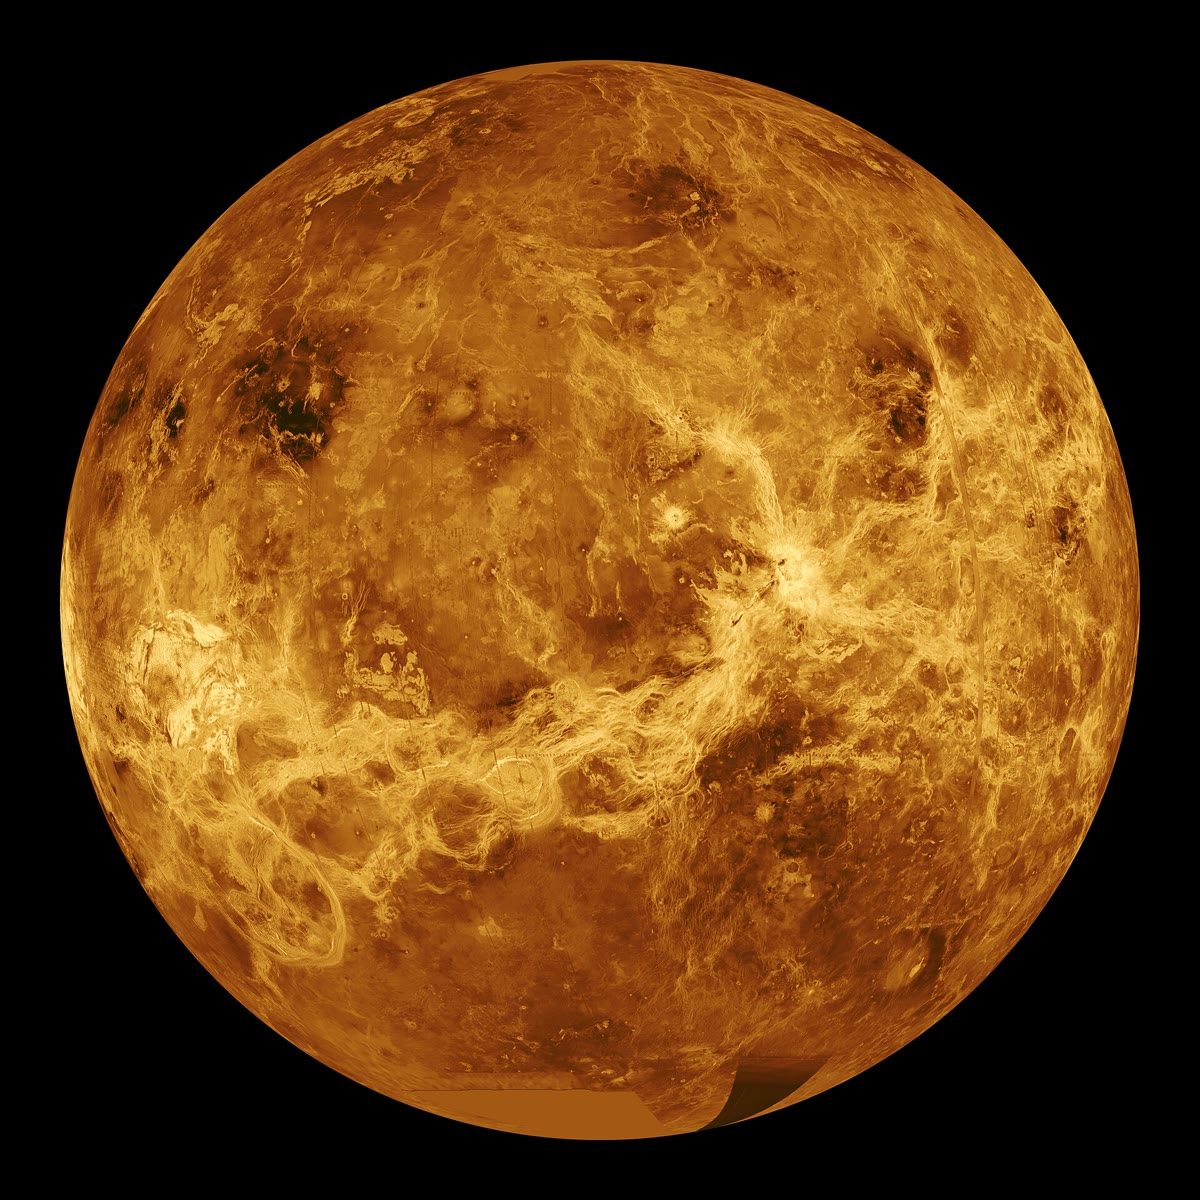
\includegraphics[width=\linewidth]{images/book3/b1-venus-radar-globe.jpg}
\end{minipage}\hspace{0.06\linewidth}
\begin{minipage}{0.4\linewidth}
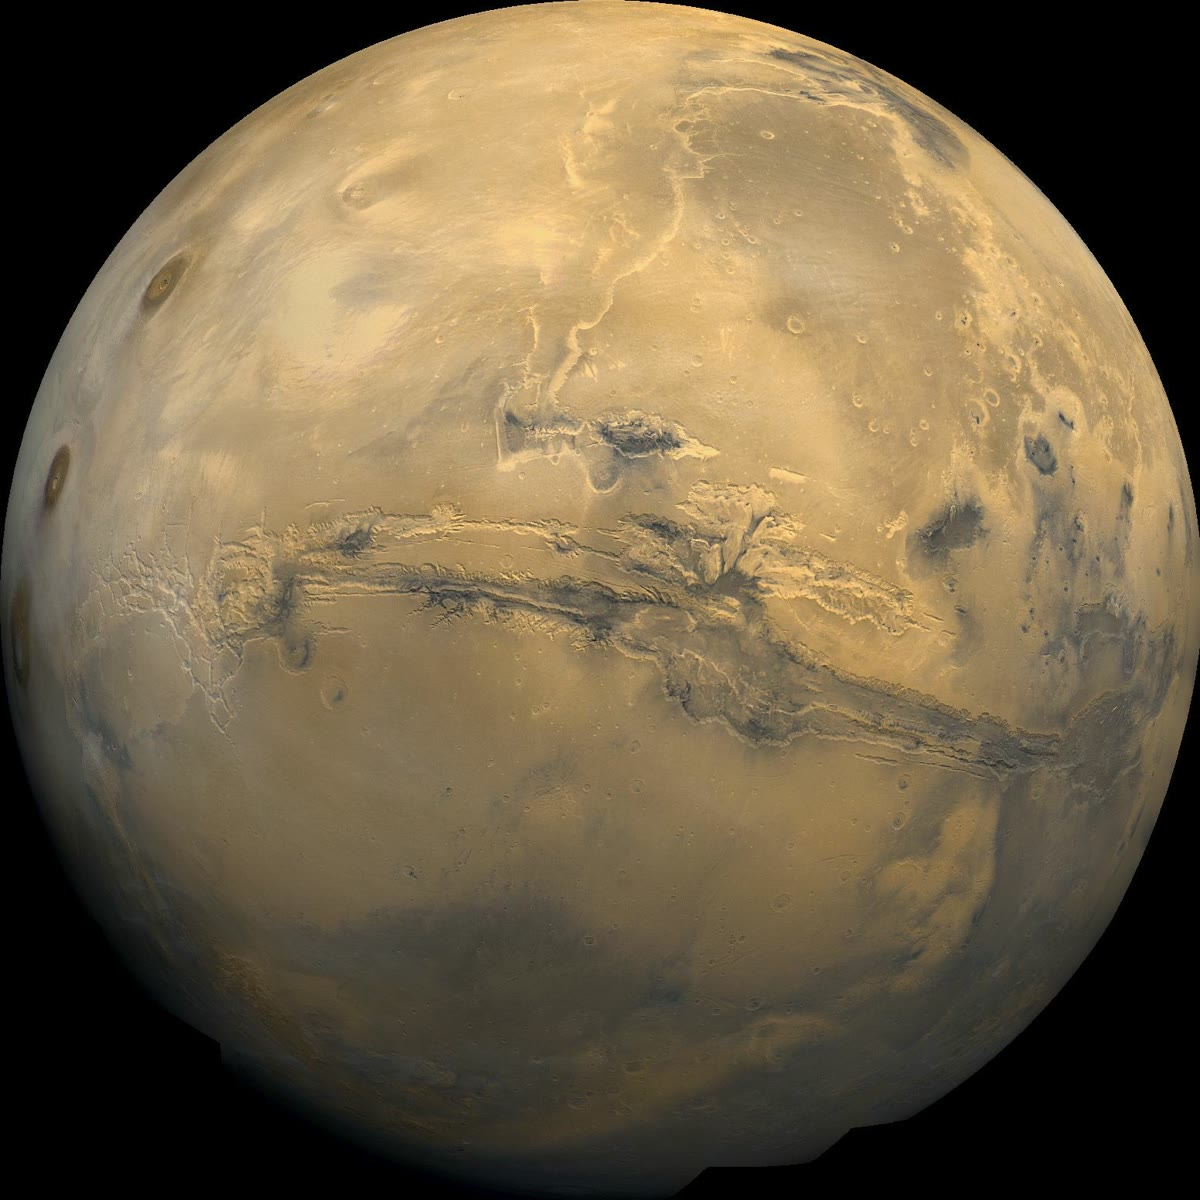
\includegraphics[width=\linewidth]{images/book3/b1-mars-valles-marineris.jpg}
\end{minipage}

{\small Kiri: permukaan Venus yang terlihat melalui awannya oleh radar wahana Magellan, dipetakan pada globe hasil simulasi komputer (warnanya disimulasikan). Kanan: Mars dari orbiter Viking 1, mosaik yang berpusat pada sistem ngarai Valles Marineris. NASA/JPL dan NASA/USGS, domain publik.}
% ledger: commons:venus-globe, commons:mars-valles
\end{omfigure}

Permukaan menyimpan catatan tentang apa yang membentuknya. Kawah tumbukan menumpuk pada setiap permukaan yang terpapar angkasa, sehingga permukaan yang sangat berkawah, seperti sebagian besar permukaan Bulan atau Merkurius, sudah tua, dan permukaan dengan sedikit kawah telah diperbarui: oleh aliran lava, oleh erosi, atau oleh lempeng-lempeng yang membawa dasar samudra Bumi kembali ke dalam mantel. Dataran vulkanik dan gunung api ditemukan pada semua \omterm{def:b1:comparative-planetology:planet-types}{planet terestrial}. Sesar, rift, dan sabuk terlipat menunjukkan bahwa litosfer Venus dan Mars telah mengalami deformasi; tetapi dari semua planet, hanya Bumi yang hari ini menunjukkan litosfer yang pecah menjadi lempeng-lempeng yang bergerak sebagai blok kaku, dengan punggungan tempat ia terbentuk dan palung tempat ia tenggelam. Mengapa hanya Bumi yang memiliki tektonik lempeng masih diperdebatkan; keberadaan air, yang melemahkan batuan, adalah salah satu alasan yang diajukan.

\section{Bulan dan benda-benda kecil}

Bulan, seperempat diameter Bumi, besar untuk sebuah satelit. Massa jenisnya, \qty{3340}{kg.m^{-3}}, mendekati batuan mantel Bumi, dan \omterm{def:b1:comparative-planetology:moi}{faktor momen inersianya}, mendekati $0.4$, menunjukkan bahwa ia paling banyak memiliki inti besi kecil. Planet-planet raksasa memiliki sistem bulan yang merupakan dunia tersendiri (lihat foto di bawah). Io, bulan besar terdalam dari empat bulan besar Jupiter, adalah dunia yang paling aktif secara vulkanik di Tata Surya, dengan ratusan gunung api, dipanaskan oleh pasang surut yang ditimbulkan Jupiter di dalamnya; vulkanisme memperbarui permukaannya lebih cepat daripada tumbukan dapat meninggalkan kawah besar. Europa, bermassa jenis \qty{3010}{kg.m^{-3}}, adalah batuan di bawah kerak es, dan ada bukti kuat tentang samudra asin di bawah kerak itu. Ganymede dan Callisto, bermassa jenis \num{1940} dan \qty{1830}{kg.m^{-3}}, tersusun dari batuan dan es dalam jumlah yang sebanding. Titan, bulan terbesar Saturnus, adalah satu-satunya bulan dengan atmosfer padat, sebagian besar nitrogen dengan sedikit metana, dan satu-satunya dunia selain Bumi yang memiliki sungai, danau, dan laut di permukaannya --- berisi metana cair dan etana; ia mungkin juga menyembunyikan samudra air.
% ledger: planet:Moon.diameter, planet:Earth.diameter, planet:Moon.density, nasa:moon, nasa:io-facts, nasa:europa, nasa:europa-facts, nasa:ganymede, nasa:titan-facts

\begin{omfigure}
\begin{minipage}{0.4\linewidth}
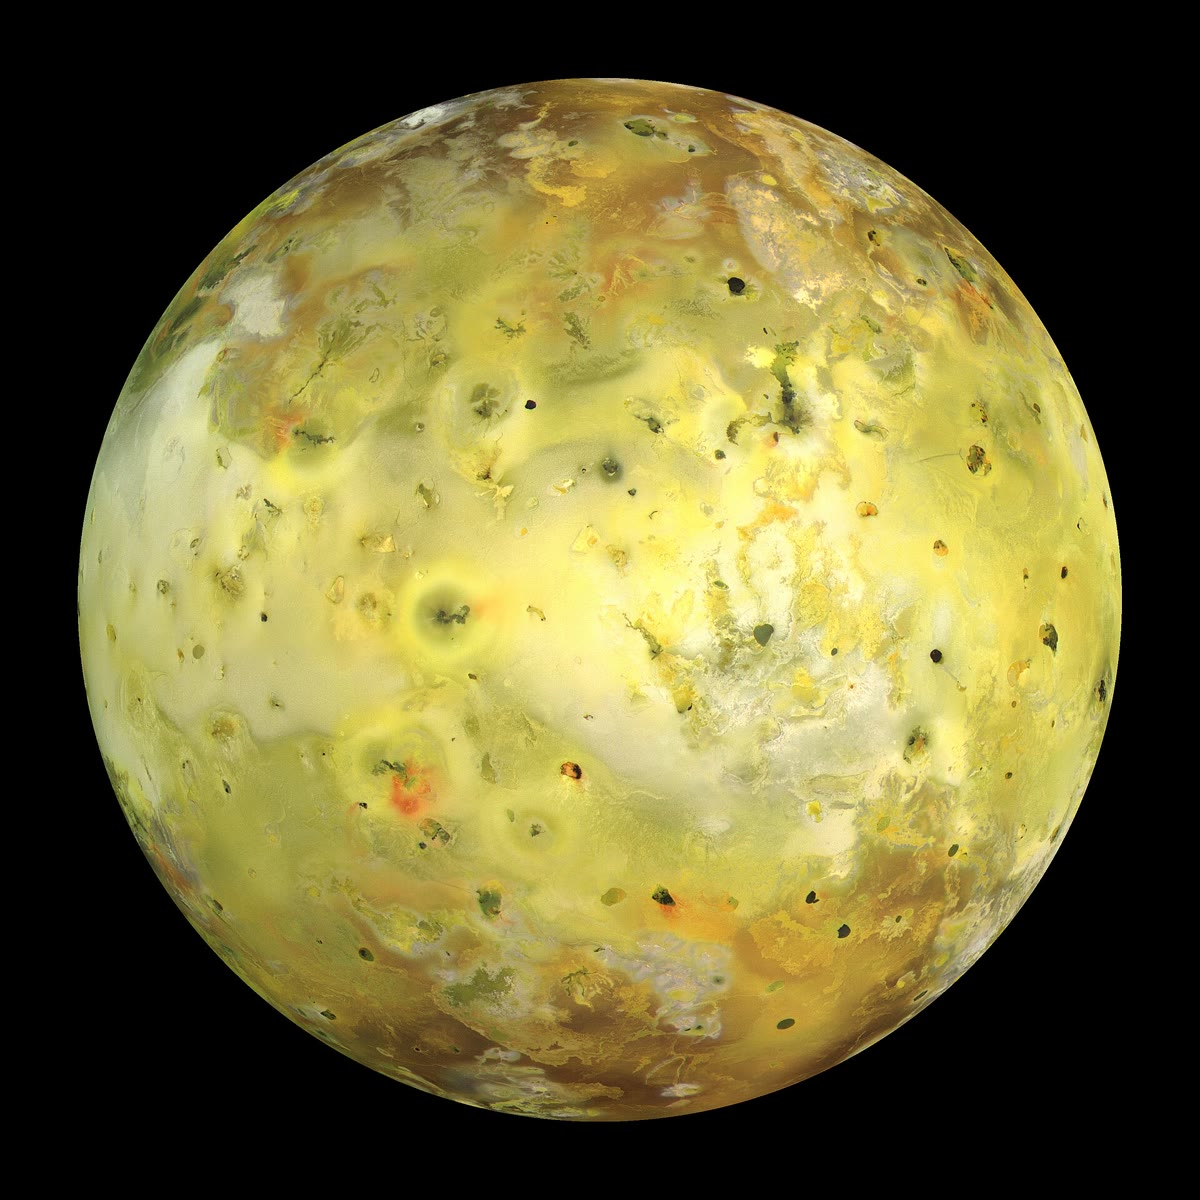
\includegraphics[width=\linewidth]{images/book3/b1-io.jpg}
\end{minipage}\hspace{0.06\linewidth}
\begin{minipage}{0.4\linewidth}
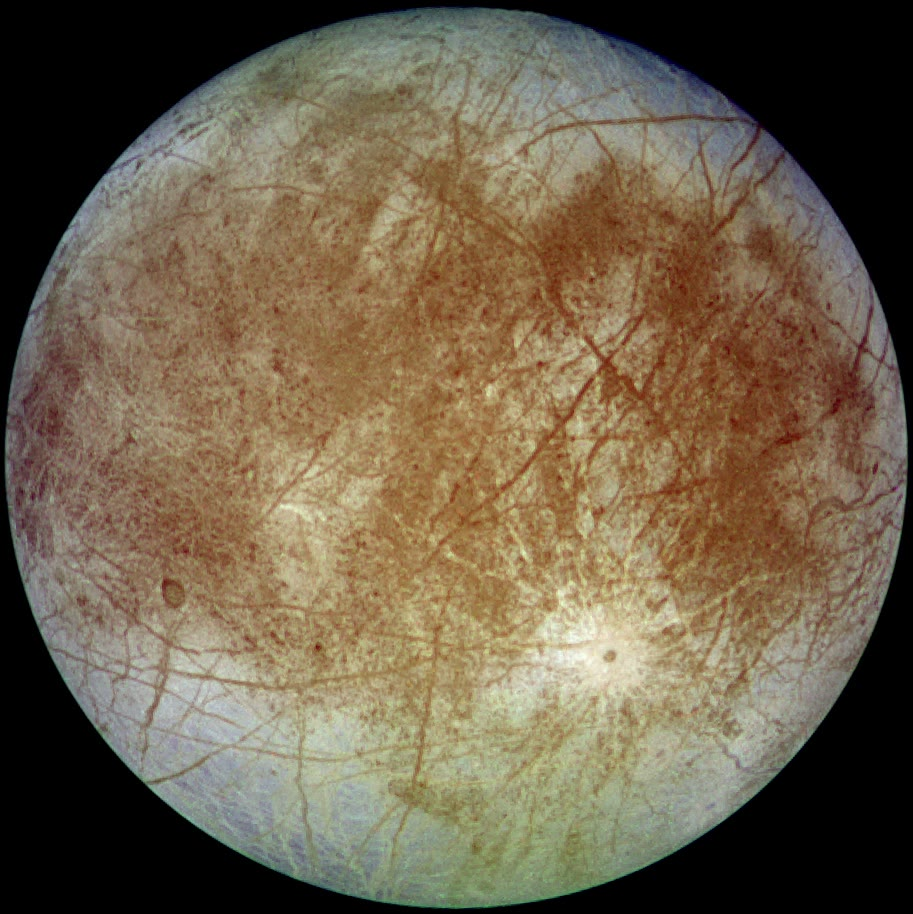
\includegraphics[width=\linewidth]{images/book3/b1-europa.jpg}
\end{minipage}

{\small Dua bulan besar Jupiter yang dilihat oleh wahana Galileo. Kiri: Io, permukaannya bertitik-titik dengan pusat vulkanik dan diwarnai oleh senyawa belerang dan lava. Kanan: Europa dalam warna alami yang mendekati; garis-garis gelap panjang adalah retakan pada kerak esnya. NASA/JPL/University of Arizona dan NASA/JPL/DLR, domain publik.}
% ledger: commons:io, commons:europa, nasa:io-facts, nasa:europa
\end{omfigure}

\begin{definition}[Asteroid, komet, objek trans-Neptunus]\label{def:b1:comparative-planetology:small-bodies}
Yang disebut \emph{asteroid}\index{asteroid} adalah benda kecil berbatu atau logam yang mengorbit Matahari, terlalu kecil untuk disebut planet dan tanpa selubung gas dan debu seperti komet; sebagian besar mengorbit di antara Mars dan Jupiter. Yang disebut \emph{komet}\index{komet} adalah benda kecil dari es dan debu yang, ketika orbitnya membawanya dekat Matahari, melepaskan gas dan debu yang membentuk selubung berpendar di sekelilingnya serta ekor yang menjauhi Matahari. Yang disebut \emph{objek trans-Neptunus}\index{objek trans-Neptunus} adalah benda Tata Surya yang orbitnya, rata-rata, berada di luar orbit Neptunus.
\end{definition}

\omterm{def:b1:comparative-planetology:small-bodies}{Objek trans-Neptunus} di Sabuk Kuiper, zona berbentuk cakram di luar Neptunus, adalah benda es dan batuan yang tersisa dari pembentukan planet-planet; Pluto, yang digolongkan sebagai planet kerdil sejak 2006, adalah salah satunya. \omterm{def:b1:comparative-planetology:small-bodies}{Asteroid} adalah puing-puing dari wilayah tempat tidak ada planet yang terbentuk. Pecahan \omterm{def:b1:comparative-planetology:small-bodies}{asteroid}, dan beberapa dari Bulan dan Mars, jatuh ke Bumi sebagai meteorit. Mereka adalah satu-satunya sampel dunia lain yang ada di tangan kita selain yang dibawa pulang oleh wahana antariksa, dan sebagian di antaranya hampir tidak berubah sejak Tata Surya terbentuk; klasifikasinya, serta apa yang mereka katakan tentang komposisi Bumi dan umur Tata Surya, adalah pokok bahasan volume Sarjana Tahun ke-2.
% ledger: nasa:pluto-facts

\section{Latihan}

\begin{exercise}[$\star$]\label{exo:b1:comparative-planetology:1}
Jupiter memiliki massa \qty{1898.13e24}{kg} dan jari-jari rata-rata \qty{69911}{km}. Hitunglah massa jenis rata-ratanya dan bandingkan dengan massa jenis air, \qty{1000}{kg.m^{-3}}.
\end{exercise}

\begin{exercise}[$\star$]\label{exo:b1:comparative-planetology:2}
Dengan memakai gambar massa jenis dan jari-jari, golongkan Merkurius, Saturnus, Uranus dan Venus sebagai \omterm{def:b1:comparative-planetology:planet-types}{planet terestrial}, \omterm{def:b1:comparative-planetology:planet-types}{raksasa gas}, atau \omterm{def:b1:comparative-planetology:planet-types}{raksasa es}, dan benarkan setiap pilihan dengan jari-jari dan massa jenisnya.
\end{exercise}

\begin{exercise}[$\star$]\label{exo:b1:comparative-planetology:3}
Venus menerima \qty{2601.3}{W.m^{-2}} dan memiliki \omterm{def:b1:comparative-planetology:albedo}{albedo Bond} 0.77. Hitunglah \omterm{def:b1:comparative-planetology:equilibrium-temperature}{suhu kesetimbangannya}. Mengapa suhu itu lebih rendah daripada suhu Bumi, meskipun Venus lebih dekat ke Matahari?
\end{exercise}

\begin{exercise}[$\star$]\label{exo:b1:comparative-planetology:4}
Urutkan Bulan ($C = 0.394$), Mars (0.366), Bumi (0.3308), Jupiter (0.254) dan Saturnus (0.210) dari yang paling seragam sampai yang paling terkonsentrasi di pusatnya. Berapakah $C$ untuk planet yang seluruh massanya terkumpul di satu titik di pusatnya?
\end{exercise}

\begin{exercise}[$\star\star$]\label{exo:b1:comparative-planetology:5}
Titan mengorbit Saturnus pada $a = \qty{1221.87e3}{km}$ dalam \num{15.945421} hari. Hitunglah massa Saturnus dan bandingkan dengan nilai tabel \qty{568.32e24}{kg}.
\end{exercise}

\begin{exercise}[$\star\star$]\label{exo:b1:comparative-planetology:6}
Bumi menerima \qty{1361}{W.m^{-2}} pada jarak \qty{149.6e6}{km} dari Matahari. Hitunglah iradiansi di Mars (\qty{228.0e6}{km}) dan di Jupiter (\qty{778.5e6}{km}), dan bandingkan dengan nilai tabel \qty{586.2}{W.m^{-2}} dan \qty{50.26}{W.m^{-2}}.
\end{exercise}

\begin{exercise}[$\star\star$]\label{exo:b1:comparative-planetology:7}
Tunjukkan bahwa, untuk albedo tertentu, $T_\mathrm{eq}$ bervariasi sebagai $d^{-1/2}$. Hitunglah $T_\mathrm{eq}$ untuk Jupiter ($S = \qty{50.26}{W.m^{-2}}$, $A = 0.343$). Jika ditemukan bahwa Jupiter memancarkan daya lebih banyak daripada yang diserapnya dari Matahari, apa implikasinya bagi bagian dalamnya?
\end{exercise}

\begin{exercise}[$\star\star$]\label{exo:b1:comparative-planetology:8}
Hitunglah pemanasan rumah kaca $T_\mathrm{surf} - T_\mathrm{eq}$ Venus (\qty{737}{K}), Bumi (\qty{288}{K}, $A = 0.294$) dan Mars (\qty{214}{K}). Nyatakan masing-masing sebagai pecahan dari $T_\mathrm{eq}$.
\end{exercise}

\begin{exercise}[$\star\star$]\label{exo:b1:comparative-planetology:9}
Untuk bola seragam, tunjukkan bahwa $C = 0.4$ dengan mengintegralkan momen inersia kulit-kulit bola tipis (sebuah kulit berjari-jari $r$ dan bermassa $\mathrm dm$ memiliki $\mathrm dI = \tfrac23 r^2\,\mathrm dm$). Berapakah nilai untuk kulit bola berongga berjari-jari $R$?
\end{exercise}

\begin{exercise}[$\star\star\star$]\label{exo:b1:comparative-planetology:10}
Merkurius memiliki $\bar\rho = \qty{5429}{kg.m^{-3}}$, $C = 0.35$ dan jari-jari \qty{2439.7}{km}. Dengan massa jenis mantel \qty{3300}{kg.m^{-3}}, pakailah model dua lapis untuk mencari jari-jari intinya, massa jenis intinya, dan pecahan massanya di dalam inti. Apa yang luar biasa tentang Merkurius?
\end{exercise}

\begin{exercise}[$\star\star\star$]\label{exo:b1:comparative-planetology:11}
Modelkan benda tak beratmosfer yang belahan siangnya bersuhu seragam $T_1$ dan belahan malamnya $T_2$, yang bersama-sama memancarkan daya yang diserap. (a) Tunjukkan bahwa jika $T_1^4 + T_2^4 = 2T_\mathrm{eq}^4$, suhu rata-ratanya $(T_1 + T_2)/2$ tidak melebihi $T_\mathrm{eq}$, dengan kesamaan hanya bila $T_1 = T_2$. (b) Untuk Bulan, $T_\mathrm{eq} = \qty{270}{K}$; ambil $T_2 = \qty{100}{K}$. Hitunglah $T_1$ dan suhu rata-ratanya.
\end{exercise}

\begin{exercise}[$\star\star\star$]\label{exo:b1:comparative-planetology:12}
Venus memiliki jari-jari \qty{6051.8}{km}, gravitasi permukaan \qty{8.9}{m.s^{-2}} dan tekanan permukaan \qty{92}{bar}. Hitunglah massa atmosfernya, bandingkan dengan massa atmosfer Bumi, \qty{5.1e18}{kg}, dan dengan massa Venus, \qty{4.8673e24}{kg}. Apa yang disarankan perbandingan itu tentang tempat karbon dioksida Bumi disimpan?
% ledger: earth:Matm, planet:Venus.gravity, nasa:venus
\end{exercise}

\section{Soal: Menimbang dan menyelidiki Mars}

\begin{problem}[{Soal akhir pekan --- massa Mars dari bulannya, massa jenis dan suhunya, serta ukuran intinya}]
\label{pb:b1:comparative-planetology:1}
% ledger: nasa:phobos, nasa:mars, nasa:mars-core, const:G, const:sigma, earth:psurf, earth:gmean, planet:Mars.Prot, planet:Earth.density
% numbers computed in the scratch calculator calc/ch03.py from the rounded data
Phobos, bulan yang lebih besar dari Mars, mengorbit pada jarak rata-rata \qty{9378}{km} dari pusat Mars dalam \num{0.31891} hari. Mars memiliki jari-jari rata-rata \qty{3389.5}{km}, periode rotasi \qty{24.6}{h}, \omterm{def:b1:comparative-planetology:moi}{faktor momen inersia} $C = 0.366$, \omterm{def:b1:comparative-planetology:albedo}{albedo Bond} 0.250, dan tekanan permukaan rata-rata \qty{6.36}{mbar}; ia menerima \qty{586.2}{W.m^{-2}} dari Matahari, dan suhu permukaan rata-ratanya sekitar \qty{214}{K}. Phobos memiliki massa \qty{1.06e16}{kg}. Ambil $G = \qty{6.6743e-11}{m^3.kg^{-1}.s^{-2}}$ dan $\sigma = \qty{5.6704e-8}{W.m^{-2}.K^{-4}}$.

\medskip
\noindent\textbf{Bagian I --- Menimbang Mars.}
\begin{enumerate}
  \item Ubahlah periode Phobos ke detik.
  \item Hitunglah $GM$ untuk Mars.
  \item Turunkan massa Mars.
  \item Apakah benar mengabaikan massa Phobos?
  \item Hitunglah kelajuan orbit Phobos.
  \item Bandingkan periode Phobos dengan rotasi Mars. Ke arah mana Phobos melintasi langit Mars?
\end{enumerate}

\medskip
\noindent\textbf{Bagian II --- Massa jenis dan gravitasi.}
\begin{enumerate}[resume]
  \item Hitunglah volume Mars.
  \item Hitunglah massa jenis rata-ratanya, dibulatkan ke \qty{10}{kg.m^{-3}}.
  \item Bandingkan dengan massa jenis Bumi, \qty{5514}{kg.m^{-3}}. Berikan dua alasan mengapa Bumi lebih padat.
  \item Hitunglah gravitasi di permukaan Mars.
  \item Hitunglah kecepatan lepas dari permukaan Mars.
\end{enumerate}

\medskip
\noindent\textbf{Bagian III --- Suhu dan atmosfer.}
\begin{enumerate}[resume]
  \item Hitunglah \omterm{def:b1:comparative-planetology:equilibrium-temperature}{suhu kesetimbangan} Mars.
  \item Bandingkan dengan suhu permukaan rata-rata. Seberapa besar pemanasan rumah kacanya?
  \item Hitunglah massa atmosfer di atas setiap meter persegi Mars, dan bandingkan dengan Bumi ($p = \qty{1014}{hPa}$, $g = \qty{9.82}{m.s^{-2}}$).
  \item Hitunglah massa total atmosfer Mars.
  \item Atmosfer Mars \qty{95}{\percent} karbon dioksida, namun pemanasan rumah kacanya kecil. Usulkan alasannya.
\end{enumerate}

\medskip
\noindent\textbf{Bagian IV --- Inti Mars.}
\begin{enumerate}[resume]
  \item Berapakah $C$ jika Mars seragam? Apa yang diberitahukan oleh nilai terukurnya?
  \item Tuliskan massa jenis rata-rata Mars dua lapis dalam jari-jari inti relatif $x$, massa jenis mantel $\rho_m$ dan massa jenis inti $\rho_c$.
  \item Tuliskan \omterm{def:b1:comparative-planetology:moi}{faktor momen inersianya} dengan besaran yang sama.
  \item Tunjukkan bahwa $x^2 = (\tfrac52C\bar\rho - \rho_m)/(\bar\rho - \rho_m)$.
  \item Dengan massa jenis rata-rata dari soal 8 dan $\rho_m =
        \qty{3500}{kg.m^{-3}}$, hitunglah $x$ dan massa jenis inti.
  \item Berapa pecahan massa Mars yang berada di intinya?
  \item Ulangi soal 21 dengan $\rho_m = 3450$ dan \qty{3550}{kg.m^{-3}}. Apa yang disimpulkan tentang ketelitian model?
  \item Berikan jari-jari inti Mars dari model dengan $\rho_m = \qty{3500}{kg.m^{-3}}$, dan bandingkan dengan nilai tabel planet, \qty{1830}{km}, serta dengan hasil seismik terbaru, \qty{1650}{km} sampai \qty{1675}{km}.
\end{enumerate}
\end{problem}
